\documentclass[a4paper, 12pt]{article}
\usepackage[a4paper, margin=2.5cm]{geometry} % Margins
\usepackage{amsmath, amssymb}
\usepackage{graphicx}
\usepackage{hyperref}
\usepackage{float}
\usepackage{color}
\usepackage{subcaption}
\usepackage{fancyhdr}
\usepackage{tcolorbox} % For boxed environment
\usepackage{setspace}


% Header and footer setup
\pagestyle{fancy}
\fancyhf{}
\fancyhead[L]{\textbf{Deep Learning – Homework 1}}
\fancyhead[R]{Group 14}
\fancyfoot[C]{\thepage}

% Title and author customization
\title{\textbf{Deep Learning (IST, 2024-25) \\ Homework 1}}
\author{Luís Calado - 103883 \& Salvador Florêncio - 102706}
\date{}

\begin{document}

\maketitle
\vspace{-0.8cm}
\begin{center}
    \textbf{Group 14}
\end{center}

%\vspace{0.1 cm}

% Contribution box
\begin{tcolorbox}[colframe=black, colback=white, sharp corners, boxrule=1pt, width=\textwidth]

\textbf{IMPORTANT:} Both members of the group were involved in the resolution of all questions in the homework.
\end{tcolorbox}

%\vspace{1cm}

\maketitle

\section*{Question 1}

\subsection*{1.a)} The performances with accuracy as the chosen metric were the following: 0.5598 on the training set, 0.3868 on the validation set and 0.3743 on the test set.
\vspace{-0.2 cm}
\begin{figure}[H]
    \centering
    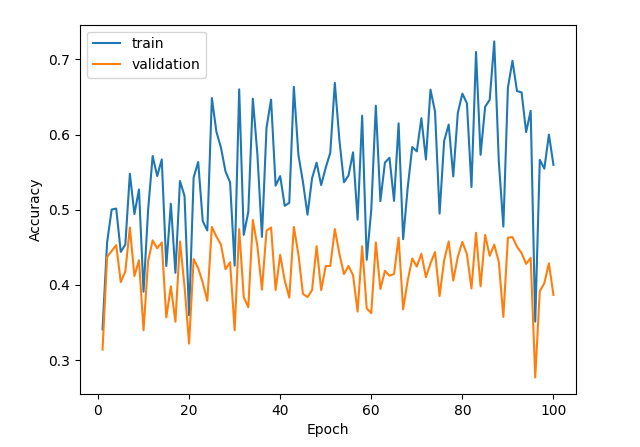
\includegraphics[width=1\textwidth]{plot/q1_1a.png}
    \caption{Perceptron: Train and validation accuracies as a function of the epoch number.}
\end{figure}

\subsection*{2.a) \& 2.b)}

Without $\ell_2$ regularization ($\lambda$ = \texttt{l2\_penalty} = $0.0$), the final test accuracy was 0.4597. With $\ell_2$ regularization ($\lambda$ = \texttt{l2\_penalty} = $0.01$), the final test accuracy was 0.5053.
\vspace{-0.5cm}

\begin{figure}[H]
    \centering
    % First subplot
    \begin{subfigure}{0.47\textwidth}
        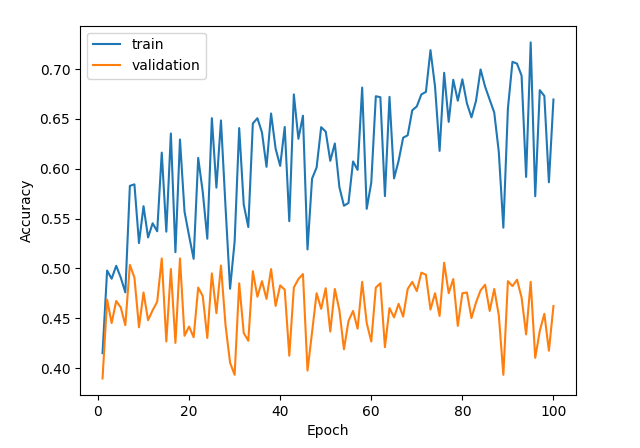
\includegraphics[width=\textwidth]{plot/q1_2a.png}
        \label{fig:without_reg}
    \end{subfigure}
    \hfill
    % Second subplot
    \begin{subfigure}{0.47\textwidth}
        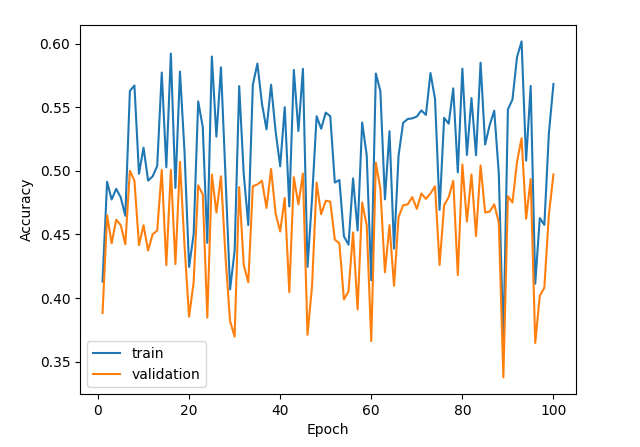
\includegraphics[width=\textwidth]{plot/q1_2b.png}
        \label{fig:with_reg}
    \end{subfigure}
    % Main caption for the entire figure
    \vspace{-0.6cm}
    \caption{Logistic regression train and validation accuracy plots as a function of the epoch number (non-regularized version and $\ell_2$-regularized versions). On the left: train and validation accuracies obtained with a non-regularized version of logistic regression. On the right: train and validation accuracies obtained with an $\ell_2$-regularized version ($\lambda=0.01$).}
    \label{fig:logistic_accuracy}
\end{figure}

%\textcolor{red}{colocar texto com o comentario}
The $\ell_2$-regularized version exhibits more stable and consistent train and validation accuracies across the epochs, whereas the non-regularized version shows more volatility, with large fluctuations throughout the training process. The improved performance and stability of the $\ell_2$-regularized version suggests that the regularization technique was effective in this case, likely helping to prevent overfitting and improve the model's generalization ability.

\subsection*{2.c)}
\vspace{-0.5 cm}
\begin{figure}[H]
    \centering
    \begin{subfigure}[b]{0.47\linewidth}
        \centering
        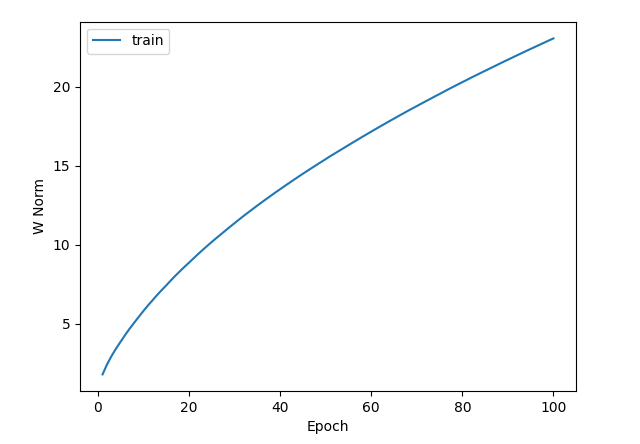
\includegraphics[width=\linewidth]{plot/q1_2a_ii.png}
        %\caption{Enter Caption for the first figure}
        \label{fig:q1_2a_ii}
    \end{subfigure}
    \hfill
    \begin{subfigure}[b]{0.47\linewidth}
        \centering
        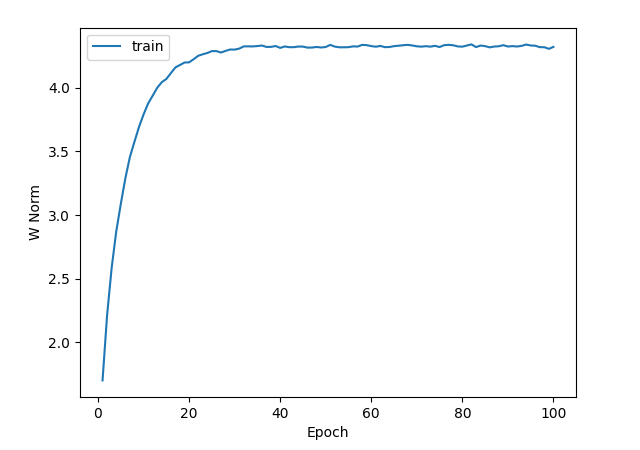
\includegraphics[width=\linewidth]{plot/q1_2b_ii.png}
        %\caption{Enter Caption for the second figure}
        \label{fig:q1_2b_ii}
    \end{subfigure}
    \vspace{-0.4 cm}
    \caption{The $\ell_2$-norm of the
weights of both the non-regularized and regularized versions of the logistic regression classifiers as a function of the epoch number. On the left: $\ell_2$-norm of the
weights obtained with a non-regularized version of logistic regression. On the right: $\ell_2$-norm of the
weights obtained with a regularized version.}
    \label{fig:side_by_side}
\end{figure}

The plots show that in the non-regularized model, the $\ell_2$-norm of the weights increases steadily (almost nearly !), indicating unbounded weight growth. This can lead to overfitting. In contrast, with $\ell_2$-regularization, the weight growth stabilizes early ($\sim$ 30th epoch), keeping the weights smaller. In the latter, the regularization term discourages large weights by penalizing their magnitude in the loss function.

\subsection*{2.d)}

Both $\ell_1$-norm and $\ell_2$-norm promote smaller weights, but $\ell_1$-norm also promotes sparser weights. Therefore, at the end of training, the values of some weights would be strictly zero (sparse).

In this way $\ell_1$ regularization would simplify the model and improve its interpretability by reducing the coefficients of the less important features to zero. This means only the most important features would have non-zero weights, effectively performing feature selection. In contrast, $\ell_2$ regularization penalizes weights proportionally to their magnitude, which tends to shrink weights towards zero but rarely makes them exactly zero (figure \ref{fig:l1_vs_l2}).
\begin{figure}[H]
    \centering
    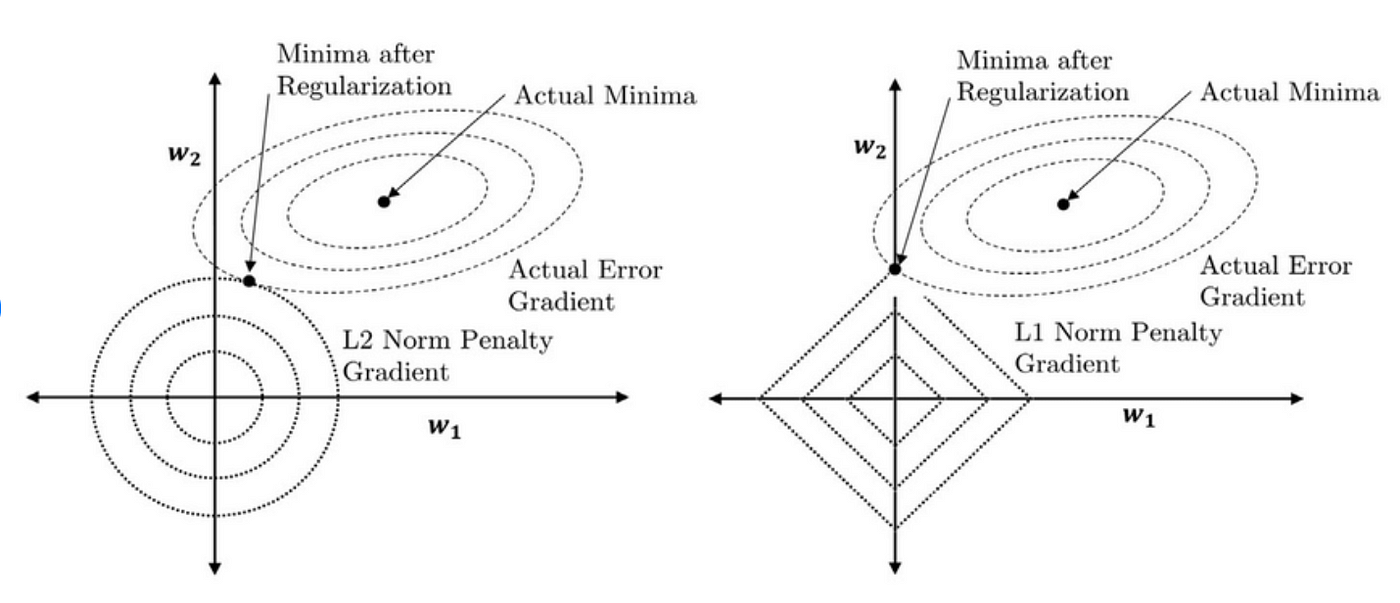
\includegraphics[width=0.7\linewidth]{plot/l1_vs_ls.png}
    \caption{Estimation of minima after regularization for \(\ell_2\)-norm (left) and \(\ell_1\)-norm (right) regularization. Geometric representation for a weight vector with two components \((w_1, w_2)\), highlighting the effects of regularization penalties on the optimization landscape. \cite{inbook}}
    \label{fig:l1_vs_l2}
\end{figure}

\subsection*{3.a)} The final test accuracy was 0.5300. The train loss and train and validation accuracies as a function of the epoch number are shown below. 
\vspace{-0.4 cm}
\begin{figure}[H]
    \centering
    % First subplot
     \begin{subfigure}{0.47\textwidth}
        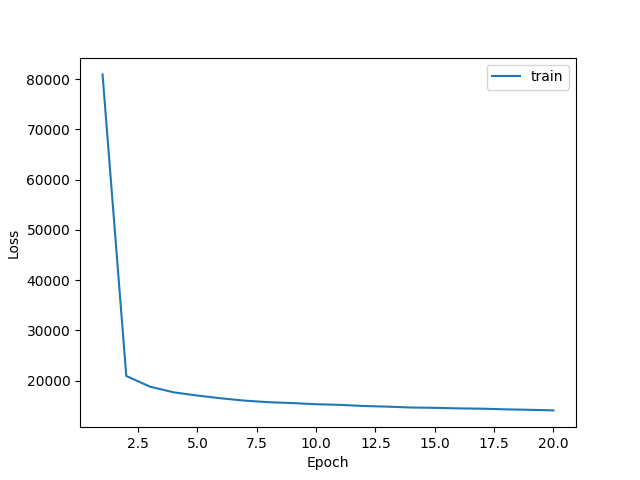
\includegraphics[width=\textwidth]{plot/1-3_losses.png}
        \label{fig:3_ii}
    \end{subfigure}
    \hfill
    \begin{subfigure}{0.43
    \textwidth}        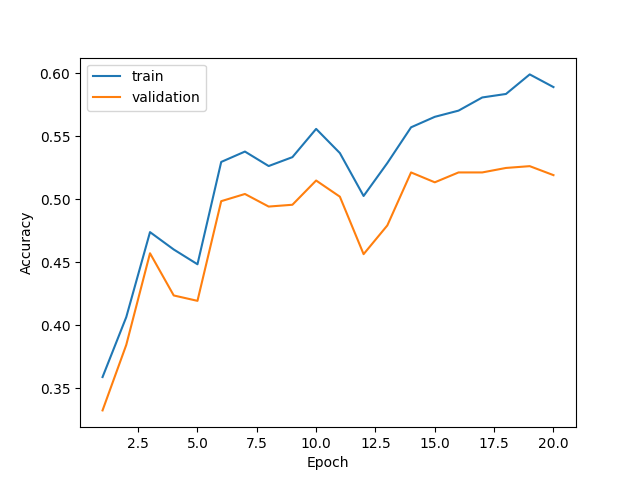
\includegraphics[width=\textwidth]{plot/1-3_accuracies.png}
        \label{fig:3_ieg}
    \end{subfigure}
    % Main caption for the entire figure
    \vspace{-0.6cm}
    \caption{On the left: train loss as a function of the epoch number. On the right: train and validation accuracies as a function of the epoch number.}
    \label{fig:q3}
\end{figure}


\section*{Question 2}
\subsection*{1.}
The \underline{best configuration} was obtained with a $lr = 0.001$ and the accuracies were 0.5264 on the validation set and 0.5247 on the test set.
\begin{figure}[H]
    \centering
    % First subplot
     \begin{subfigure}{0.30\textwidth}
        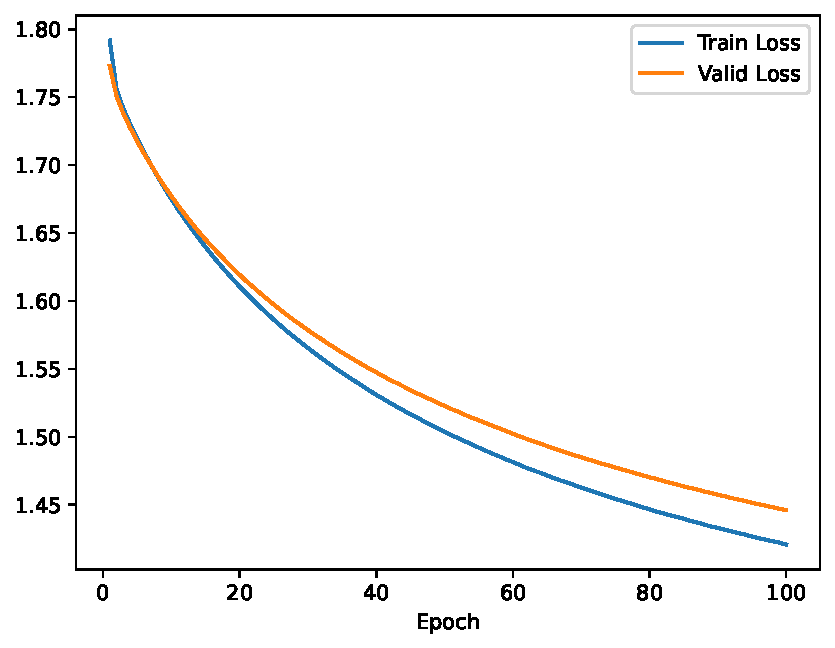
\includegraphics[width=\textwidth]{plot/logistic_regression-training-loss-batch-32-lr-1e-05-epochs-100-l2-0.01-opt-sgd.pdf}
        \label{fig:lr_0.00001}
    \end{subfigure}
    \hfill
    \begin{subfigure}{0.30
    \textwidth}
        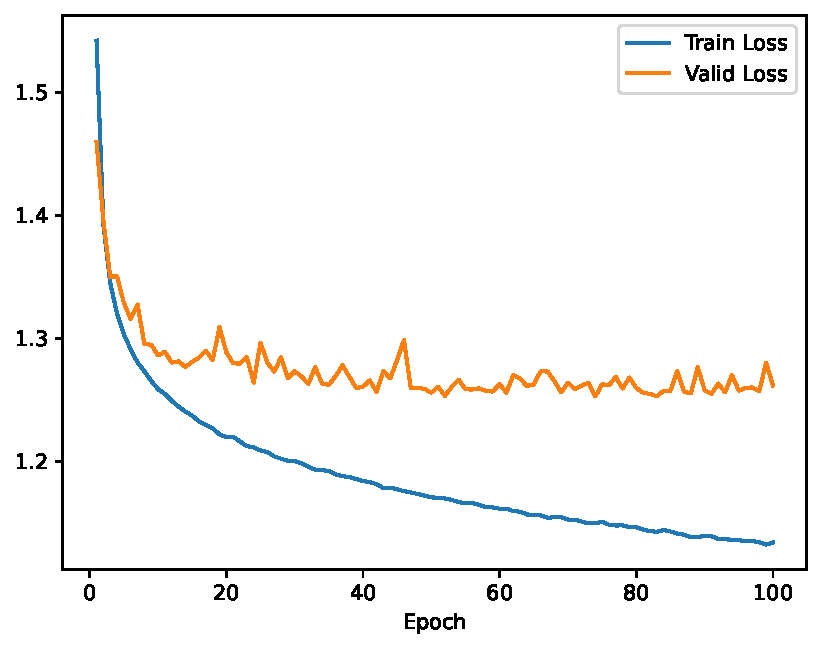
\includegraphics[width=\textwidth]{plot/logistic_regression-training-loss-batch-32-lr-0.001-epochs-100-l2-0.01-opt-sgd.pdf}
        \label{fig:lr_0.001}
    \end{subfigure}
    \hfill
    \begin{subfigure}{0.30
    \textwidth}
        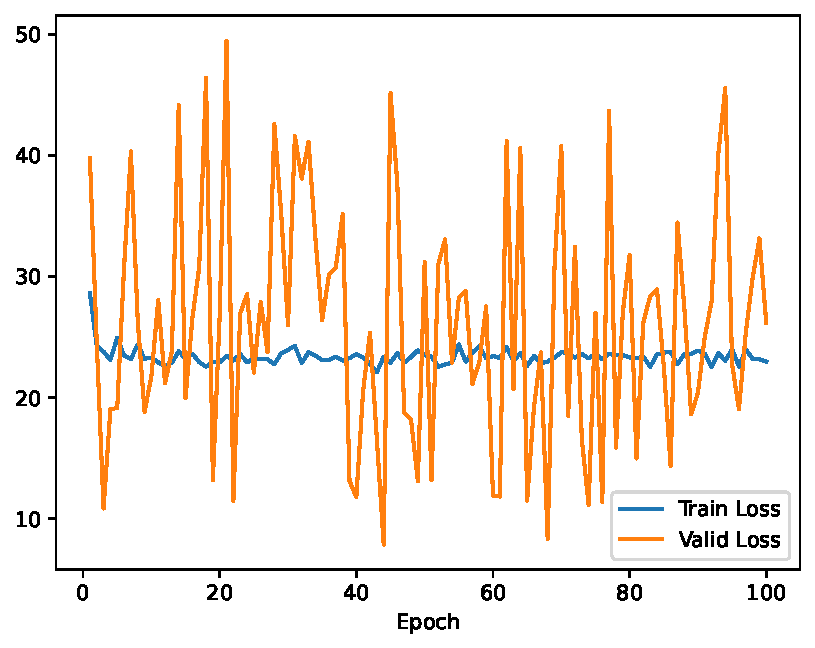
\includegraphics[width=\textwidth]{plot/logistic_regression-training-loss-batch-32-lr-0.1-epochs-100-l2-0.01-opt-sgd.pdf}
        \label{fig:lr_0.01}
    \end{subfigure}
    % Main caption for the entire figure
    \vspace{-0.6cm}
    \caption{Training and validation loss curves over 100 epochs for different learning rates: \(lr = 0.00001\) (left), \(lr = 0.001\) (middle), and \(lr = 0.1\) (right).}
    \label{fig:q2_1}
\end{figure}

%\textcolor{red}{Adicionar accuracies dos outros modelos com diferentes learnig rates}
For a $lr = 0.00001$ the accuracies were 0.4694 on the validation set and 0.4623 on the test set. And for a $lr = 0.1$ the accuracy on the validation set was 0.4558 and 0.4693 on the test set.  

\begin{itemize}
    \item $lr = 0.00001$: Validation loss decreases steadily but very slowly, expressing a similar behaviour to the training loss. This indicates that a very small learning rate value results in slow convergence, leading to underfitting.
\end{itemize}
\begin{itemize}
    \item $lr = 0.001$: Validation loss decreases rapidly and stabilizes, suggesting effective training. So by using a well-balanced value for the learning rate, we allow the model to converge efficiently without overfitting or instability over the epochs.
\end{itemize}
\begin{itemize}
    \item $lr = 0.1$: Validation loss fluctuates wildly, showing instability due to an excessively high learning rate value. Suggesting that a very high learning rate causes the model to overshoot the optimal point, leading to erratic loss behavior and poor generalization.
\end{itemize}

We can conclude that the performance is directly affected by the learning rates. One possible reason for the performance to be bad when the learning rate is equal to 0.1 is because this particular learning rate is just too big for this model, which causes the algorithm to overshoot the optimal weights and diverge. For $lr \in \{0.00001,0.01\}$  the model seems to be a good fit, as the loss plots decrease then begin to stabilize, and they have the best values of validation accuracy and test accuracy. When the learning rate is equal to 0.00001 it’s possible to notice from the loss plots that the model is clearly underfit: this may be because the
network is converging too slowly.

\subsection*{2. a)}

For a \texttt{batch\_size} of 64, the final validation accuracy was 0.6068, test accuracy was 0.6083, and execution time was 4 minutes and 6 seconds. In contrast, for a \texttt{batch\_size} of 512, the final validation accuracy was 0.5028, test accuracy was 0.5190, and execution time was only 2 minutes and 20 seconds. 

\begin{figure}[H]
    \centering
    % First subplot
     \begin{subfigure}{0.47\textwidth}
        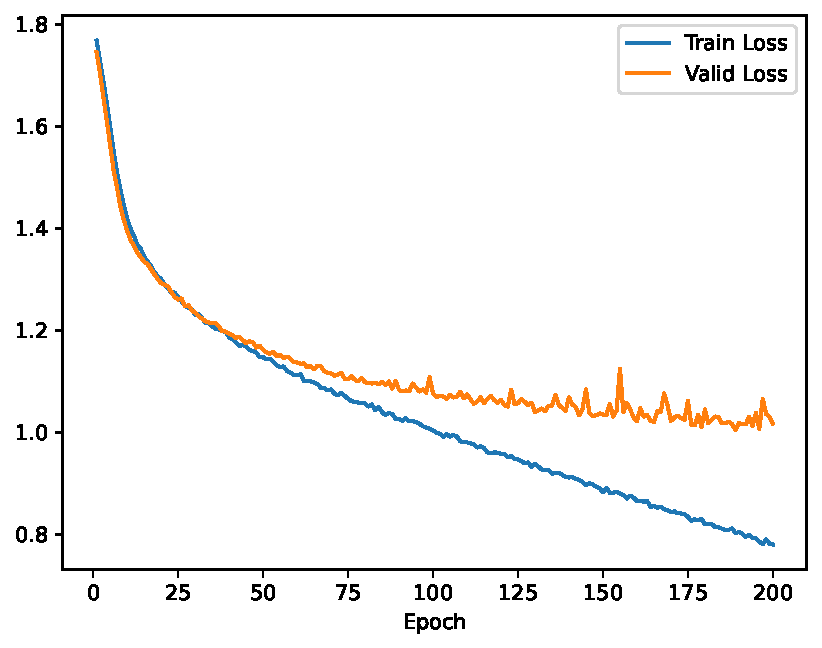
\includegraphics[width=\textwidth]{plot/mlp-training-loss-batch-64-lr-0.002-epochs-200-hidden-200-dropout-0.3-l2-0.0-layers-2-act-relu-opt-sgd-mom-0.0.pdf}
        \label{fig:3_ii}
    \end{subfigure}
    \hfill
    \begin{subfigure}{0.47
    \textwidth}
        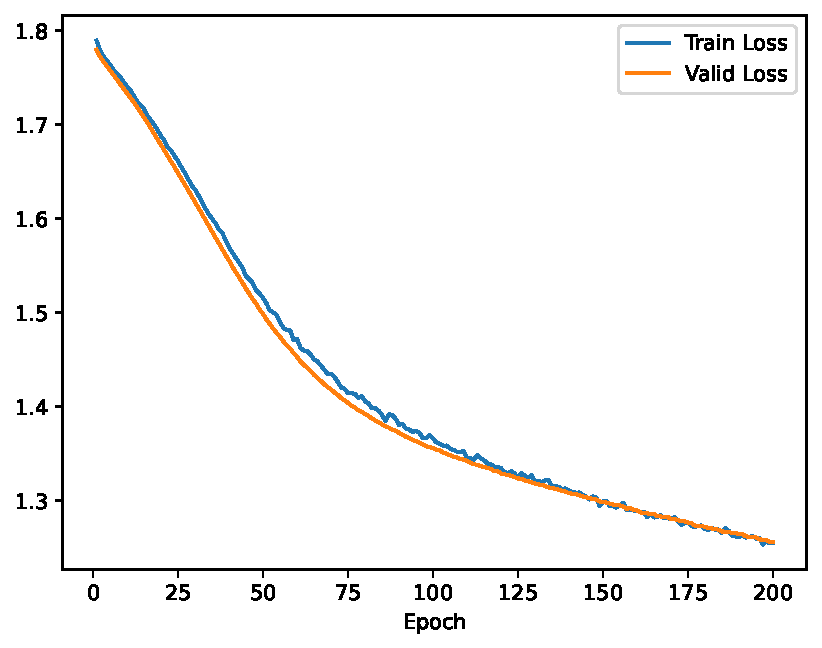
\includegraphics[width=\textwidth]{plot/mlp-training-loss-batch-512-lr-0.002-epochs-200-hidden-200-dropout-0.3-l2-0.0-layers-2-act-relu-opt-sgd-mom-0.0.pdf}
        \label{fig:3_ieg}
    \end{subfigure}
    % Main caption for the entire figure
    \vspace{-0.6cm}
    \caption{Train and validation losses as a function of the epoch number. On the left: \texttt{batch\_size} = 64. On the right: \texttt{batch\_size} = 512. }
    \label{fig:q3}
\end{figure}

Despite the longer execution time, the smaller \texttt{batch\_size} of 64 achieved significantly better accuracy, tending us to believe that larger batch sizes, while faster, may lead to underfitting and reduced performance.

For a \texttt{batch\_size} of 64, the training loss steadily decreases to 0.7798, and the validation loss stabilizes around 1.0167, indicating effective learning and reasonable generalization. In contrast, with a \texttt{batch\_size} of 512, the training loss is higher ($\sim$ 1.2551), and the validation loss also remains higher ($\sim$ 1.2562), suggesting underfitting due to fewer parameter updates per epoch.

Therefore, we can conclude that smaller batch sizes (64) allow the model to capture more fine-grained updates to the weights, because they introduce some noise to the training data which prevents overfitting, and they also converge faster during training, which makes the model adapt more quickly, although being more time-consuming. While larger batch sizes (512), tend to smooth out gradients too much, potentially missing important details in the data. This can result in underfitting, as observed here.

In terms of execution time, the larger \texttt{batch\_size} reduced training time significantly but at the cost of lower accuracy and higher loss. The smaller \texttt{batch\_size} took longer to train but yielded better performance. 

\subsection*{2. b)}

\begin{figure}[H]
    \centering
    % First subplot
     \begin{subfigure}{0.30\textwidth}
        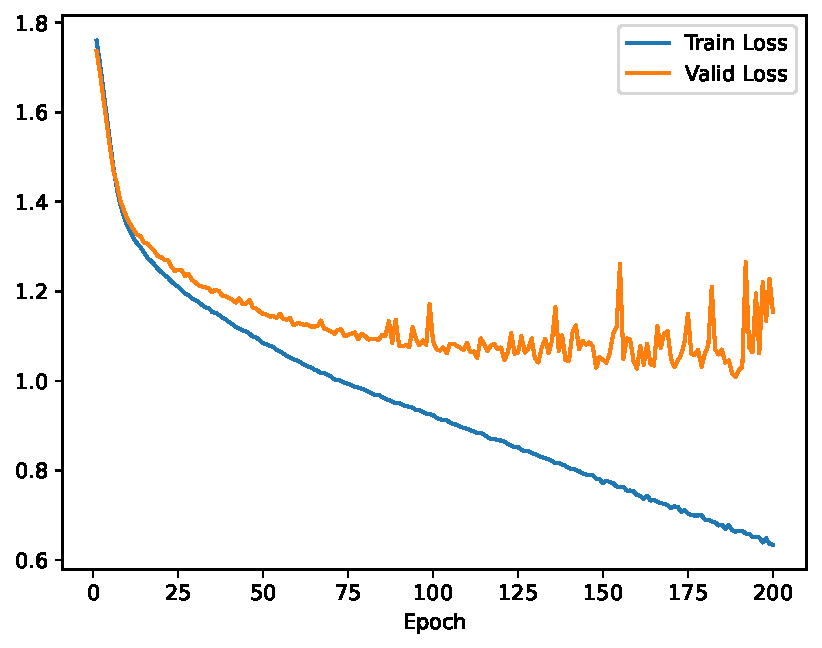
\includegraphics[width=\textwidth]{plot/mlp-training-loss-batch-64-lr-0.002-epochs-200-hidden-200-dropout-0.01-l2-0.0-layers-2-act-relu-opt-sgd-mom-0.0.pdf}
        \label{fig:lr_0.00}
    \end{subfigure}
    \hfill
    \begin{subfigure}{0.30
    \textwidth}
        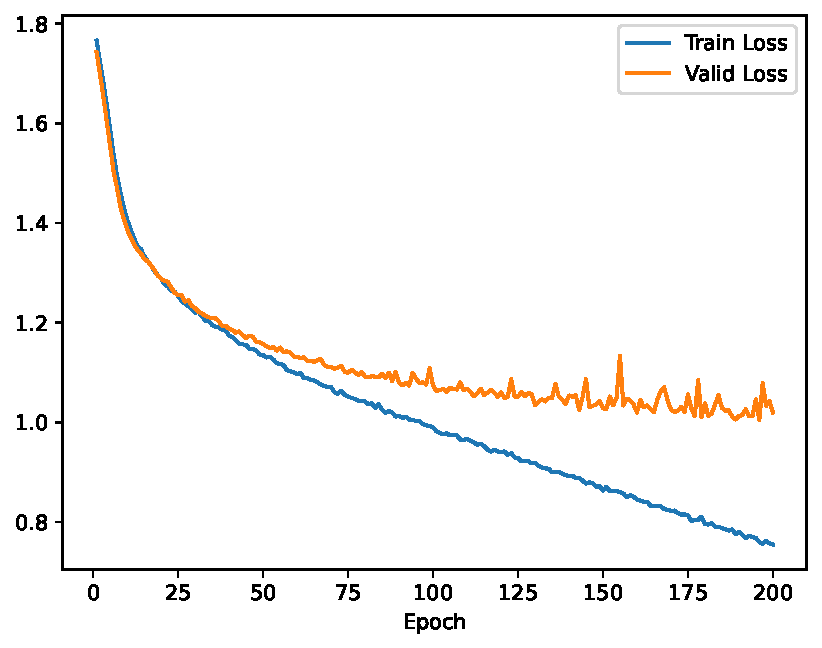
\includegraphics[width=\textwidth]{plot/mlp-training-loss-batch-64-lr-0.002-epochs-200-hidden-200-dropout-0.25-l2-0.0-layers-2-act-relu-opt-sgd-mom-0.0.pdf}
        \label{fig:lr_0}
    \end{subfigure}
    \hfill
    \begin{subfigure}{0.30
    \textwidth}
        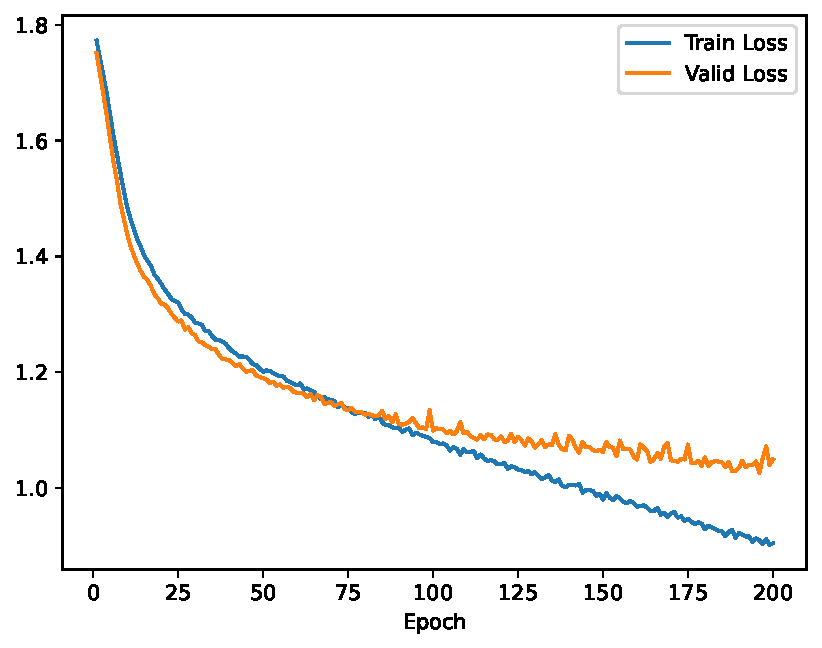
\includegraphics[width=\textwidth]{plot/mlp-training-loss-batch-64-lr-0.002-epochs-200-hidden-200-dropout-0.5-l2-0.0-layers-2-act-relu-opt-sgd-mom-0.0.pdf}
        \label{fig:lr_0.0}
    \end{subfigure}
    % Main caption for the entire figure
    \vspace{-0.6cm}
    \caption{On the left: \texttt{dropout} = 0.01. On the middle: \texttt{dropout} = 0.25. On the right: \texttt{dropout} = 0.5. Train and validation losses as a function of the epoch number.}
    \label{fig:q}
\end{figure}

%The best configuration was obtained with a \texttt{dropout} = 0.25 and the accuracies were 0.6068 on the validation set and  0.6070 on the test set. For a \texttt{dropout} = 0.01, we obtained a validation accuracy of 0.5912 and a test accuracy of 0.5833. And for a \texttt{dropout} = 0.5, accuracies of 0.5976 on the validation set and 0.5953 on the test set.

The best configuration was obtained with a \texttt{dropout} = 0.25 and the accuracies were 0.6068 on the validation set and 0.6070 on the test set. For a \texttt{dropout} = 0.01, we obtained a validation accuracy of 0.5762 and a test accuracy of 0.5763. And for a \texttt{dropout} = 0.5, accuracies of 0.5976 on the validation set and 0.5953 on the test set.

By looking at the results, we can see that a \texttt{dropout} = 0.25 achieves the best trade-off between training and validation performance, leading to the highest validation and test accuracies. While a \texttt{dropout} = 0.5 likely over-regularizes the model, preventing it from fully capturing the training data patterns, which leads to underfitting and slightly worse performance. And a \texttt{dropout} = 0.01, barely affects the network, which may result in slight overfitting since it doesn't provide sufficient regularization.

%A wider gap between training and validation losses can indicate overfitting (\texttt{dropout} = 0.01), and a too small a gap can indicate underfitting (\texttt{dropout} = 0.5).

In conclusion, \texttt{dropout} = 0.25 is the best configuration among these parameters for this model as it balances regularization effectively, achieving the highest validation and test accuracies. The results highlight the importance of tuning \texttt{dropout} to prevent overfitting while allowing the model to learn meaningful patterns from the data. By randomly selecting the percentage of the neurons not to be used, \texttt{dropout} further regularizes training by dynamically altering the network itself instead of modifying the loss function. This prevents hidden units to co-adapt to other units, forcing them to be more generally useful. Beyond regularization, \texttt{dropout} also improves model robustness by simulating diverse network configurations.

%Use this: Dropout is a form of regularization used to prevent overfitting, which consists in removing some hidden units, during training chosen at random. Each hidden unit output is set to 0 with probability $p$.
%This prevents hidden units to co-adapt to other units, forcing them to be more generally useful.
%\colorbox{red}{Analyze and explain the results.}
\subsection*{2. c)}

\begin{figure}[H]
    \centering
    % First subplot
     \begin{subfigure}{0.47\textwidth}
        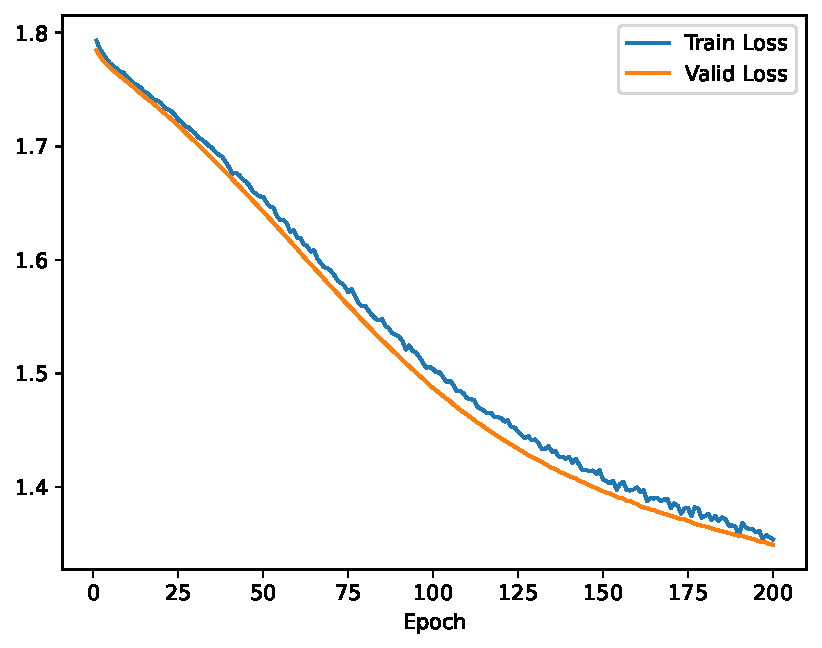
\includegraphics[width=\textwidth]{plot/mlp-training-loss-batch-1024-lr-0.002-epochs-200-hidden-200-dropout-0.3-l2-0.0-layers-2-act-relu-opt-sgd-mom-0.0.pdf}
        \label{fig:3_}
    \end{subfigure}
    \hfill
    \begin{subfigure}{0.47
    \textwidth}
        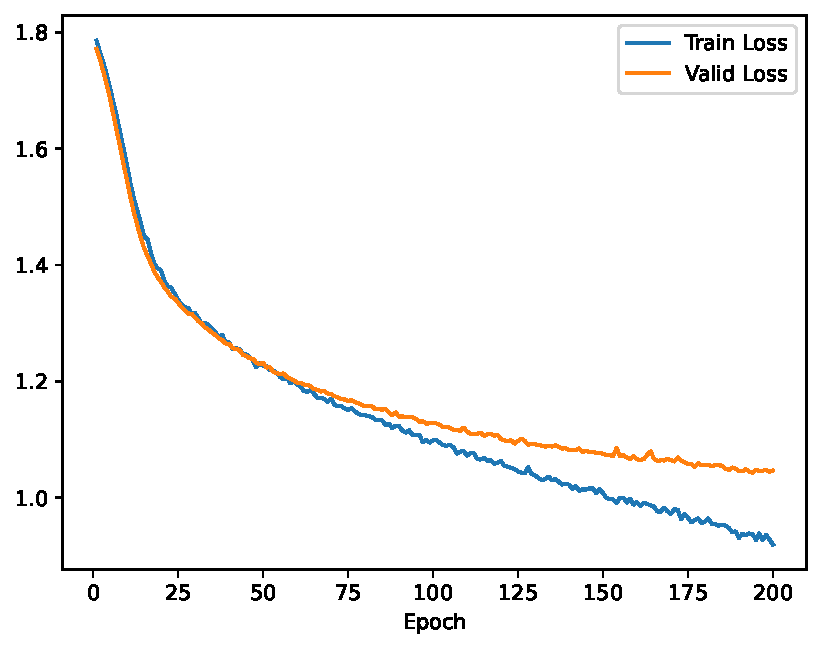
\includegraphics[width=\textwidth]{plot/mlp-training-loss-batch-1024-lr-0.002-epochs-200-hidden-200-dropout-0.3-l2-0.0-layers-2-act-relu-opt-sgd-mom-0.9.pdf}
        \label{fig:3_eg}
    \end{subfigure}
    % Main caption for the entire figure
    \vspace{-0.6cm}
    \caption{On the left: \texttt{momentum} = 0.0. On the right: \texttt{momentum} = 0.9. Train and validation losses as a function of the epoch number.}
    \label{fig:qa}
\end{figure}

For \texttt{momentum} = 0.0, we obtained a validation accuracy of 0.4701, and a test accuracy of 0.4887. In comparison, for a \texttt{momentum} = 0.9, the accuracies were 0.5997 on the validation set and 0.6017 on the test set.  We clearly see that \texttt{momentum} = 0.9 leads to higher validation and test accuracies, indicating a better overall performance.

By looking at the plots, we observe that without \texttt{momentum}, the training and validation losses decrease steadily but at a slower rate when compared to \texttt{momentum} = 0.9, where 
the model converges faster, having a more rapid decrease in both training and validation losses.

This is because \texttt{momentum} helps accelerate gradient descent by incorporating the previous steps, allowing to increase the update in directions with a stable gradient. Resulting in a faster convergence, as observed for \texttt{momentum} = 0.9.

This way, for \texttt{momentum} = 0.9, the model generalizes better and converges faster because momentum helps the optimizer "remember" past gradients. This makes it less sensitive to noise in the data (random variability in the data that can mislead the optimization) and guides it more smoothly through the optimization process.  On the other hand, without momentum (\texttt{momentum} = 0.0), the optimizer relies only on the current gradient. This results in slower learning, and a greater gap between training and validation performance, ultimately leading to lower accuracy.

Therefore, \texttt{momentum} significantly improves the performance of the model by accelerating convergence and enhancing generalization. This is evident in both the faster reduction of losses and the higher validation/test accuracies when \texttt{momentum} = 0.9 is used.

\section*{Question 3}
\subsection*{1.}
Let $i$ be the $i$th row and $j$ the $j$th column of $W$. We have
\[
    h_i = g \left(\sum_{j=1}^{D} w_{ij} x_j +b_i \right )= \left(\sum_{j=1}^{D} w_{ij} x_j +b_i \right ) \left(1-\sum_{j=1}^{D} w_{ij} x_j - b_i \right ) \tag{1}
\]
\[
= - \sum_{j=1}^{D} w_{ij} x_j \sum_{j=1}^{D} w_{ij} x_j + (1-2b_i) \sum_{j=1}^{D} w_{ij} x_j + b_i -b_{i}^2,
\] 
 Let
\[
\phi(x) =
\begin{bmatrix}
    1 \\
    x_1 \\
    \vdots \\
    x_D \\
    2x_1x_2 \\
    \vdots \\
    2x_{D-1}x_D \\
    x_{1}^2 \\
    \vdots \\
     x_{D}^2
\end{bmatrix},
\quad
a_i =
\begin{bmatrix}
    b_i - b_{i}^2  \\
    (1-2b_i) w_{i1}\\
    \vdots \\
    (1-2b_i) w_{iD} \\
    -w_{i1}w_{i2} \\
    \vdots \\
    -w_{i(D-1)}w_{iD} \\
    -w_{i1}^{2} \\
    \vdots \\
    -w_{iD}^{2}
    
\end{bmatrix},
\quad
A_\Theta =
\begin{bmatrix}
    a_1^\top \\
    \vdots \\
    a_K^\top
\end{bmatrix}.
\tag{2}
\]
We then have $h_i = a_i^\top \phi(x)$ and $h = A_\Theta \phi(x)$. Finally we may observe that $\phi(x)$ contains $ 1 + D + \frac{D(D-1)}{2} + D $ rows, which simplifies to $\frac{(D+1)(D+2)}{2}$.

\subsection*{2.}
We have \vspace{-0.5cm} \[
\hat{y} = {v}^\top {h} +v_0 ={v}^\top A_\Theta \phi(x) + v_0 = \sum_{i=1}^{K} v_{i} h_i + v_0 = \boldsymbol{v_0} + v_1h_1 + ... + v_Kh_K. \tag{3}
\]
We need to account for the $v_0$ term in the predicted output $\hat{y}$; we will take advantage of the fact that $\phi_1 (x) = 1$ is a constant.

Let 
\[
c_\Theta =
\begin{bmatrix}
    \boldsymbol{v_0}  + \sum\limits_{i=1}^{K} v_i (b_i - b_i^2) \\
    \sum\limits_{i=1}^{K} v_i (1 - 2b_i) w_{i1} \\
    \vdots \\
    \sum\limits_{i=1}^{K} v_i (1 - 2b_i) w_{iD} \\
    -\sum\limits_{i=1}^{K} v_i w_{i1}w_{i2} \\
    \vdots \\
    -\sum\limits_{i=1}^{K}v_iw_{i(D-1)}w_{iD} \\
   -\sum\limits_{i=1}^{K}v_i w_{i1}^{2} \\
    \vdots \\
    -\sum\limits_{i=1}^{K}v_i w_{iD}^{2}
\end{bmatrix} \text{with} \hspace{0.15 cm} {c}_{\Theta} \in \mathbb{R}^{\frac{(D+1)(D+2)}{2}}
,
\quad 
\phi(x) =
\begin{bmatrix}
    1 \\
    x_1 \\
    \vdots \\
    x_D \\
    2x_1x_2 \\
    \vdots \\
    2x_{D-1}x_D \\
    x_{1}^2 \\
    \vdots \\
     x_{D}^2
\end{bmatrix}
\tag{4}
\] 
The resulting model is \textbf{not} linear in $\Theta$, because $c_\Theta$ is not a linear function in terms of the original parameters $\Theta$: all entries of $c_\Theta$ are \textbf{nonlinear} on $W, b \hspace{0.15cm}\text{and} \hspace{0.15cm} v$.
\subsection*{3.}
The expression for \( c\) may be rewritten as a vector with three components, i.e., \( c = (c_1, c_2, c_3) \). Specifically, the components are defined as follows:
\[
c_1 = \boldsymbol{v_0} + \sum\limits_{i=1}^{K} v_i (b_i - b_i^2), \hspace{0.2cm}
c_2 =
\begin{bmatrix}
    \sum\limits_{i=1}^{K} v_i (1 - 2b_i) w_{i1} \\
    \vdots \\
    \sum\limits_{i=1}^{K} v_i (1 - 2b_i) w_{iD} \\
\end{bmatrix} \text{ and} \hspace{0.2cm}
c_3 = 
\begin{bmatrix}
    -\sum\limits_{i=1}^{K}v_i w_{i1}^{2} \\
    -\sum\limits_{i=1}^{K} v_i w_{i1}w_{i2} \\
    \vdots \\
    -\sum\limits_{i=1}^{K}v_iw_{i(D-1)}w_{iD} \\
    -\sum\limits_{i=1}^{K}v_i w_{iD}^{2}
\end{bmatrix}.
\tag{5}
\]
Here, a row adjustment was performed in \( c_3 \) compared to the original vector \( c_\Theta \), allowing \( c_3 \) to be expressed as \( c_3 = -\text{vech}(C) \), where \( C = W^\top \text{Diag}(v)W \) is a symmetric matrix. From $c_3$ one can recover a subset of $\Theta$: $(W,v)$. If \( K \geq D \), we can derive any \( c_{\Theta} \in \mathbb{R}^{\frac{D(D+1)}{2}} \) using the \(\text{vech}\) operation. However, if \( K < D \), an equivalent parametrization may not exist because in such a case, \(c_3\) could result in a matrix \( C \) with rank exceeding \( K \), which would prevent recovering the parameters \( (W, v) \in \mathbb{R}^{K \times D} \times \mathbb{R}^K \). To proceed with $c_2$, one can recover $b$: 
\[
c_2 = \begin{bmatrix}
w_{11} & \cdots & w_{1K}  \\
\vdots & \ddots & \vdots \\
w_{D1} & \cdots & w_{DK}
\end{bmatrix}
\begin{bmatrix}
    v_1(1-2b_1) \\
    \vdots \\
    v_K(1-2b_k)
\end{bmatrix}.
\tag{6}
\]
Lastly, one may recover $v_0$ from $c_1$, after knowing the parameter $v$: $c_1 = \boldsymbol{v_0} + \sum\limits_{i=1}^{K} v_i (b_i - b_i^2)$.
 
\subsection*{4.}
Let $X \in \mathbb{R}^{N \times \frac{(D+1)(D+2)}{2}}$ have $\phi(x_n)$ as rows, and define $\mathbf{y} = (y_1, \dots, y_N)$. We want to minimize
\[
\frac{1}{2} \| X c_\Theta - \mathbf{y} \|_F^2
\tag{7}\]
with respect to $c_\Theta$. This is a least squares problem whose solution is
\[
\hat{c}_\Theta = X^+ \mathbf{y} = (X^\top X)^{-1} X^\top \mathbf{y}.
\tag{8}\]
This is a global optimum. The assumption \( N > \frac{(D+1)(D+2)}{2} \) ensures that the matrix \( X \) has full rank, specifically \(\text{rank}(X) = \frac{(D+1)(D+2)}{2}\). This guarantees that \( X^\top X \) is invertible.
What makes our problem special is that the activation function allows for a reparametrization where the model becomes linear in terms of the transformed features $\phi(x)$. 
\bibliography{refs} 
\bibliographystyle{plain} 
\end{document}

